\documentclass[12pt]{amsart}

\addtolength{\hoffset}{-2.25cm}
\addtolength{\textwidth}{4.5cm}
\addtolength{\voffset}{-2.5cm}
\addtolength{\textheight}{5cm}
\setlength{\parskip}{0pt}
\setlength{\parindent}{15pt}

\usepackage{amsthm}
\usepackage{amsmath}
\usepackage{amssymb}
\usepackage[colorlinks = true, linkcolor = black, citecolor = black, final]{hyperref}

\usepackage{graphicx}
\usepackage{multicol}
\usepackage{ marvosym }
\usepackage{wasysym}
\usepackage{tikz}
\usetikzlibrary{patterns}

\newcommand{\ds}{\displaystyle}

\setlength{\parindent}{0in}

\pagestyle{empty}

% ----------------------------

% The "stuff" above here is called the preamble of the document.  It sets the margins and loads special packages.  Probably the only reason you would need to edit something above here would be to add a package to do something very specific... but probably everything you need is loaded already

% -----------------------------

\begin{document}

\thispagestyle{empty}

{\scshape Math 2400} \hfill {\scshape \large Center of Mass Mobile} \hfill {\scshape P3}
 
\smallskip

\hrule

\bigskip

We need some more Math Department decorations, so we're going to build a mobile that demonstrates our mastery of the concept of the center of mass of a two dimensional object.  This is partially a group effort, since the final product is a single mobile, but each participant will contribute one shape and submit their own write-up of the work.

\bigskip

\bigskip

The basic process will be:

\begin{enumerate}

\item  Design and build a cool shape.  This should be basically two-dimensional, but make sure that your shape {\bf is not} uniform density.

\medskip

\item  If you need to, put a backing (and fronting?) on your shape to ensure pieces stay together.

\medskip

\item  Find the center of mass of that object.

\medskip

\item  Test it and make sure it is reasonable.

\medskip

\item  Clearly mark the coordinates on the object itself as well as the total mass.

\medskip

\item  Attach a string to the object at the center of mass so that it will hang from the string level with the floor.

\medskip

\item  Hang your object from the mobile in a way that keeps the entire mobile balanced.

\medskip

\end{enumerate}

\bigskip

\bigskip

\bigskip

\bigskip

I have some shapes that you can use as pieces, tape, scissors, card-stock, and other helpful things available in my office for building.  Stop by to pick up some materials, or you can absolutely build from anything you've already got.  I'll maintain the mobile in my office, and have tools and materials available for hanging.  You may come by anytime to add your shape to the mobile; you don't need an appointment, but you are welcome to check with me first to make sure I'm around.  You should allow a few minutes to do the necessary computations and adjustments to keep it balanced.

The write-up you submit on Blackboard should include 
\begin{itemize}
\item  A diagram of the complete shape and all the specifications,
\item  The steps to compute the center of mass,
\item  An explanation of the computation and derivation of any new formulas, and
\item  A summary of any collaboration and computations needed to hang the final object and keep the whole system balanced.
\end{itemize}

\bigskip

\bigskip

\bigskip

\bigskip

The next page has a grid of 1 centimeter squares.  That can be helpful for tracing out your shapes, but you are not required to use it.

\newpage

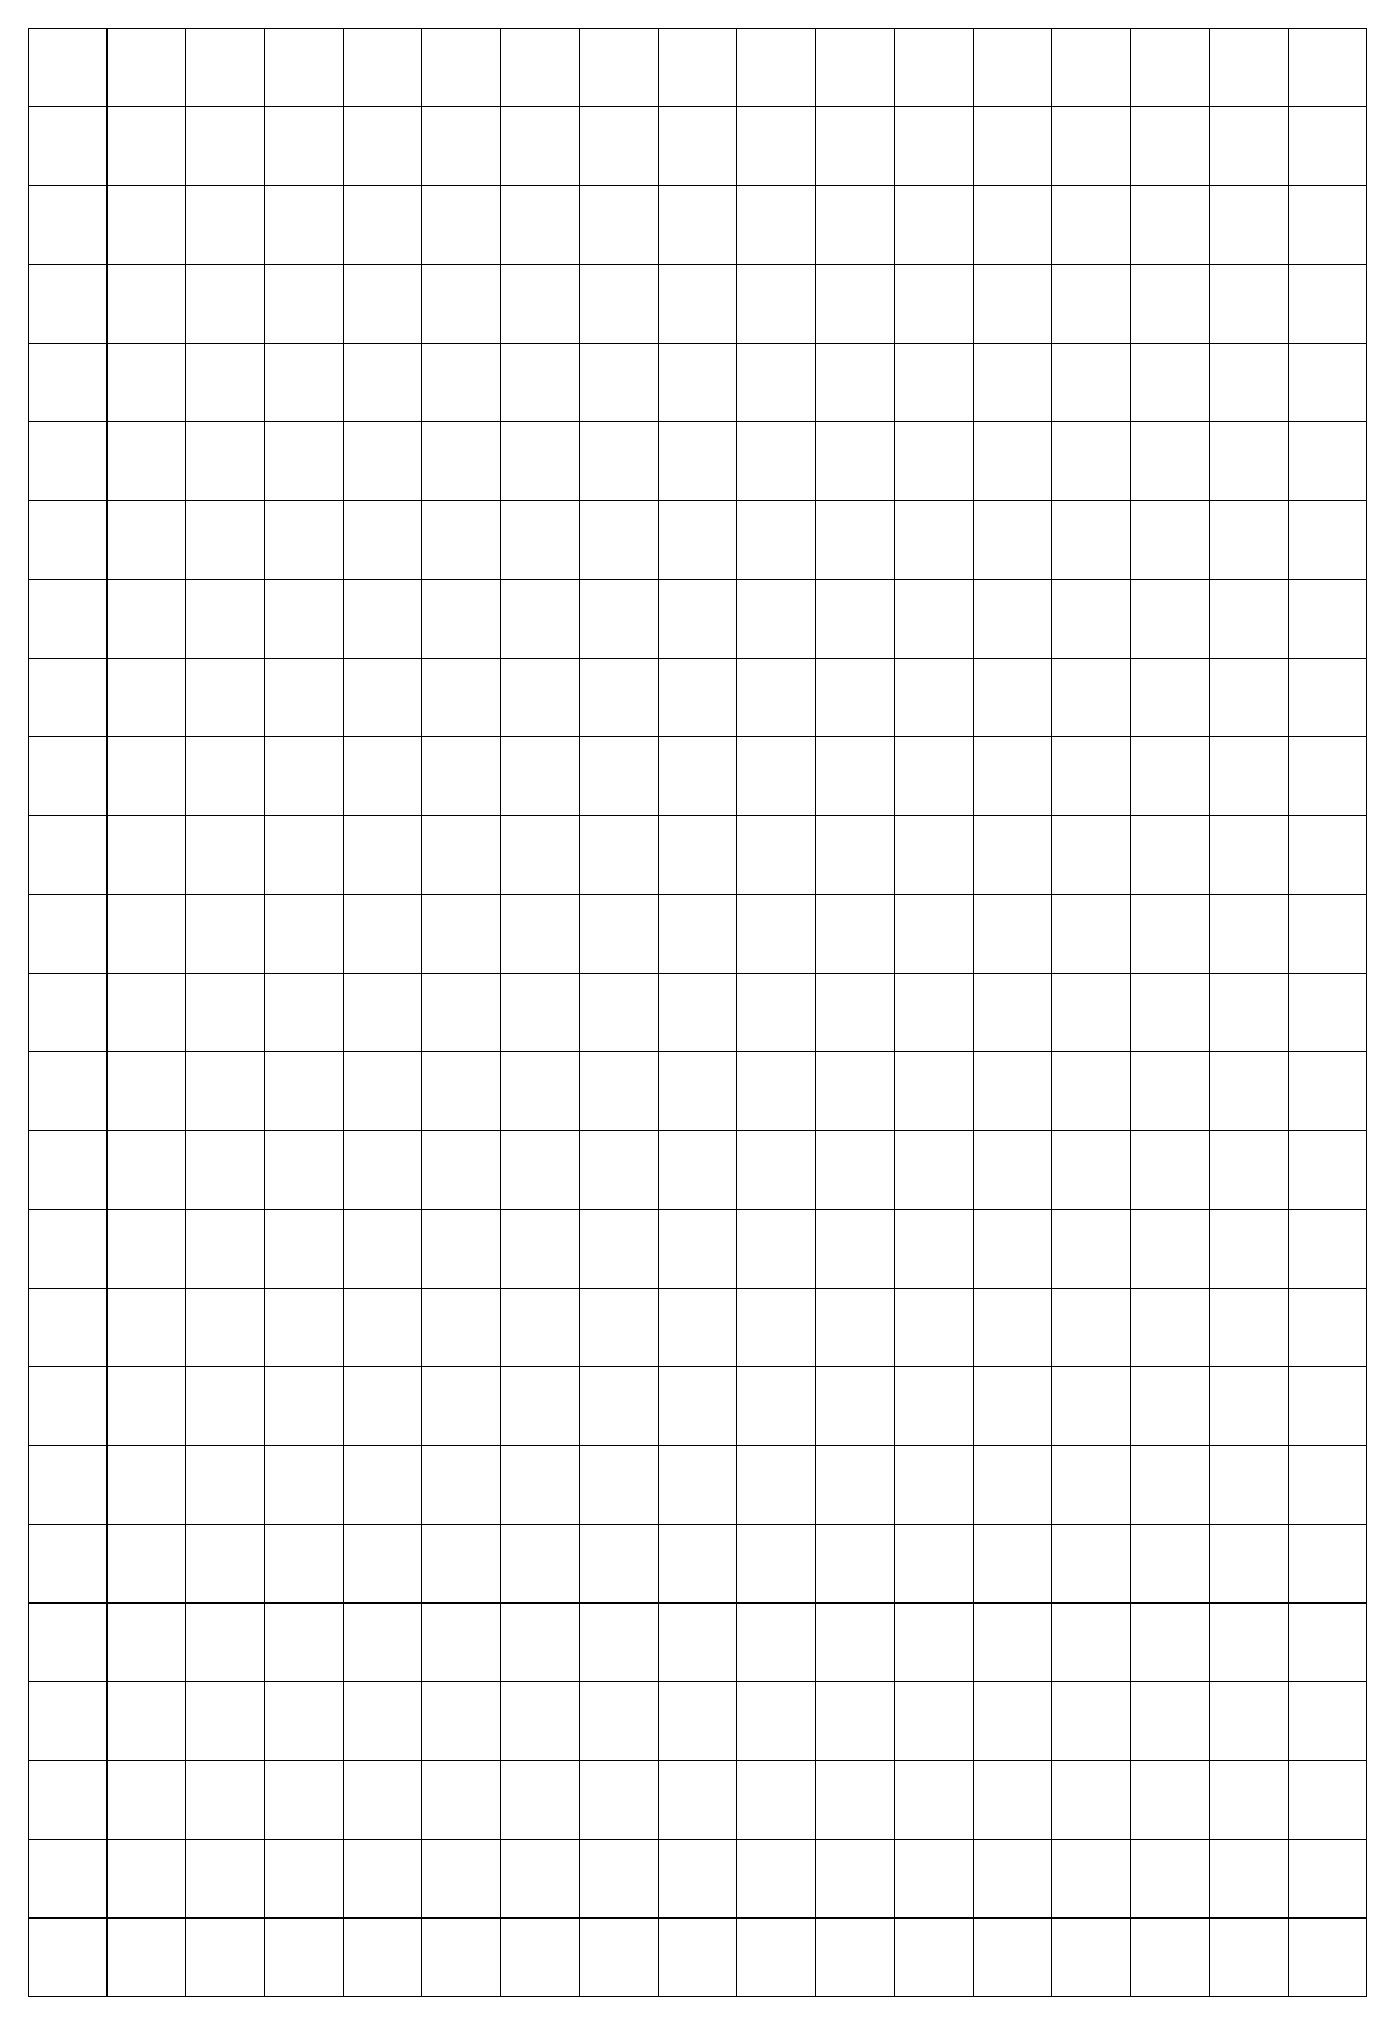
\begin{tikzpicture}
\draw (0,0) grid (17, 25);
\end{tikzpicture}

\newpage

% ------------------------------------------
%
%
%
%IF YOU WANT TO LEARN HOW TO DO SOME OF THIS YOURSELF IN LaTeX
%
%
%
%
%
%START HERE!
%
%
%
%
% This % symbol at the start of a line tells the compiler to treat the line as a comment.
% I have included some comments throughout the LaTeX code for this document to try to help you navigate some of the basic things included here.
% 
%
%
%
%
%
%
%
%
% If you're using Overleaf, at any time you can click on a place in the pdf on the right, and the corresponding portion of the code on the left will be highlighted.  That makes it easer to see find the pieces of code for the specific thing you want to be able to do.

{\scshape Math 2400} \hfill {\scshape \large Sample Solution} \hfill {\scshape P3}
 
% \scshape inside a set of {  }  makes the text appear in all caps.
% \large adjusts the size of the font
% \hfill spaces these things out evenly across the page.

% You can use other commands: \bf, \it, \underline for text as well.
% There is a similar \vspace command that will space things out vertically on the page.
 
\smallskip

\hrule

% \smallskip, \medskip, and \bigskip are another way to space things out vertically.  You can also use \vspace{1in} and change in the input according to how much space you want to add (or take away if you use a negative number.)

\bigskip

% Notice how the section is labeled and I've written in complete sentences.
{\bf The Shape:}  For my shape I chose a plastic square and a third of a circular disk.  I extended the card stock outer layer to include the triangle on the left side of the diagram above.  I measured the side of the square as well as the radius of the circle to be approximately 10cm.  After a bit of thinking, I chose to put the the origin at the lower left corner of the square to be the origin of the coordinate plane.

\bigskip


% The tikz package allows you to code diagrams.  This is not something you are expected to do, but I'm happy to help if you want to explore.
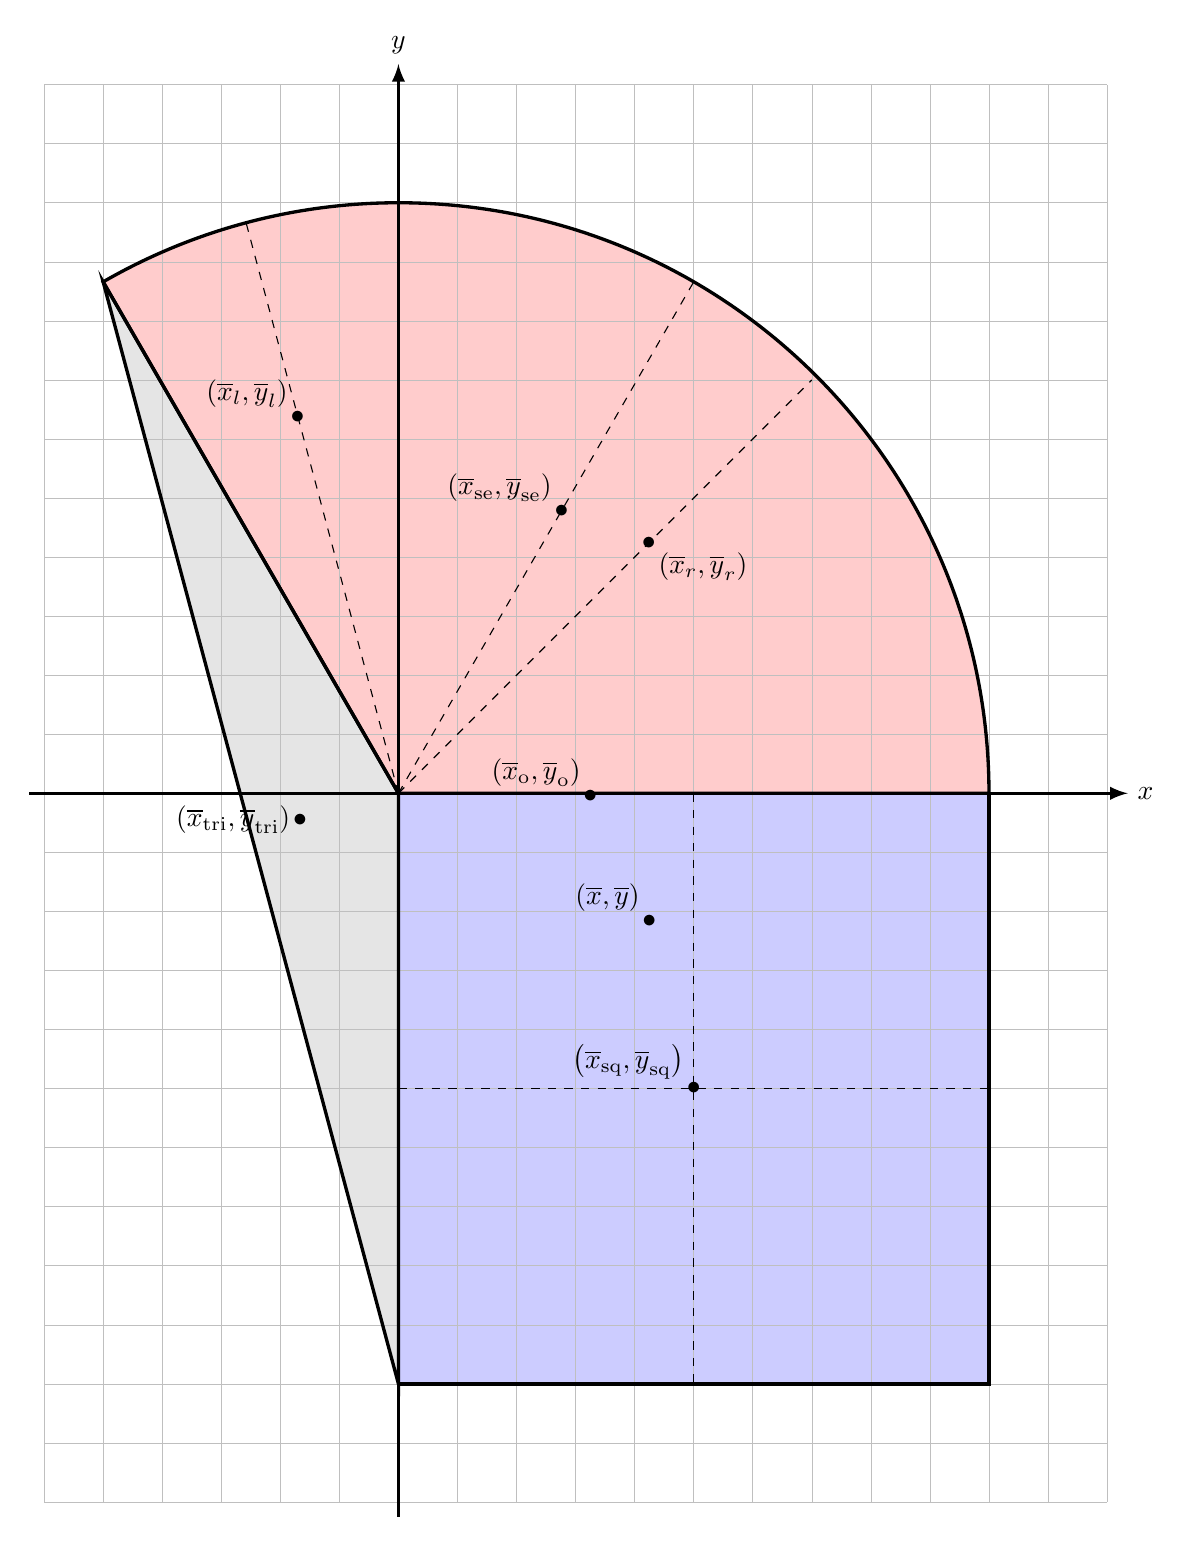
\begin{tikzpicture}[scale = .75]
\draw[fill = blue!20] (0,0) -- (10,0) -- (10,-10) -- (0, -10) -- cycle;
\draw[fill = red!20] (10,0) arc (0:120:10) -- (0,0) -- cycle;
\draw[fill = gray!20] (-5,8.66)--(0,0)--(0,-10)--cycle;
\draw[very thin, gray!50] (-6,-12) grid (12, 12);
\draw[very thick] (0,0) --(10,0) -- (10,-10) -- (0, -10) -- cycle;
\draw[very thick] (10,0) arc (0:120:10) -- (0,0) -- cycle;
\draw[very thick] (-5,8.66)--(0,0)--(0,-10)--cycle;
\node at (-1.6666666, -.45) {$\bullet$};
\node[anchor = east] at (-1.6666666, -.45) {$\left(\overline{x}_{\text{tri}}, \overline{y}_{\text{tri}}\right)$};
\node at (5, -5) {$\bullet$};
\node[anchor = south east] at (5, -5) {$\left(\overline{x}_{\text{sq}},\overline{y}_{\text{sq}}\right)$};
\node at (2.76, 4.77) {$\bullet$};
\node[anchor = south east] at (2.76, 4.77) {$\left(\overline{x}_{\text{se}},\overline{y}_{\text{se}}\right)$};
\node at (3.25, -.05) {$\bullet$};
\node[anchor = south east] at (3.25, -.05) {$\left(\overline{x}_{\text{o}},\overline{y}_{\text{o}}\right)$};
\node at (4.25, -2.16) {$\bullet$};
\node[anchor = south east] at (4.25, -2.16) {$\left(\overline{x},\overline{y}\right)$};

\node at (4.24, 4.24) {$\bullet$};
\node[anchor = north west] at (4.24, 4.24) {$(\overline{x}_r, \overline{y}_r)$};

\node at (-1.71, 6.37) {$\bullet$};
\node[anchor = south east] at (-1.71, 6.37) {$(\overline{x}_l, \overline{y}_l)$};

\draw[very thick, -latex] (-6.25, 0) -- (12.35, 0);
\node[anchor = west] at (12.35, 0) {$x$};

\draw[very thick, -latex] (0, -12.25) -- (0, 12.35);
\node[anchor = south] at (0, 12.35) {$y$};

\draw[dashed] (5, 0) -- (5, -10);
\draw[dashed] (0, -5) -- (10, -5);

\draw[dashed] (0,0) -- (5, 8.66);

\draw[dashed] (0,0) -- (7,7);

\draw[dashed] (0,0) -- (-2.59, 9.7);
\end{tikzpicture}
% Another option for images, graphs, pictures, etc. is to include a .jpg, .pdf, etc. file of the graphic.  
% In Overleaf, you need to add this file to the project.  Click on "Project" with the squares in the menu at the top. Choose "Add Files..." and probably upload from your computer. (If you have installed a LaTeX editor on your own machine, then make sure the file you want to include is in the same folder as your .tex document... or look up how to call other folders.)
% Once the file is part of the project, type the name of the file inside the {}.  You typically do not need the file type .pdf, .jpg, etc. but nothing bad happens when you include it.
% The [] can be left empty or used to enter a variety of different instructions, most commonly adjustments to the size of the image are here. You can use inches or centimeters or points, LaTeX knows many measurement systems. You can also specify relative lengths, like I have above.  \textwidth is the width of the text in this document, and putting .85 in front shrinks it to 85% of the text width.

%\begin{center}\includegraphics[width = .85\textwidth]{SampleGraph}\end{center}

\bigskip

The points and dotted lines are various centers of mass and lines of symmetry that will be discussed further as we compute things.

\newpage

{\bf The Masses:} The mass of the entire square is 28 g and the circular sector has a mass of 9 g.  To compute the mass of the card-stock outer layers, I used the scale to determine the mass of a complete file folder, which was 22 grams, and measured the dimensions of the folder to get the area of 1323 cm$^2$.  I computed the area of my entire shape:
% Anything with \begin{} needs a corresponding \end{}.  What goes inside the brackets {} is the environment you're working in.  The align* environment will keep the "&" in your work aligned in a vertical column.  This is good for lining up equals signs in long calculations. If you leave out the *, each line will be numbered.  This can be handy for referring back to later.
\begin{align*}A & = A_{\text{sq}} + A_{\text{se}} + A_{\text{tri}}\\
% The \\ tells the align* environment to move to the next line. Since align forces us into a mathematics environment, we need to specify when we want "regular" text inside align.
& = s^2 + \frac{1}{3}\pi r^2 + \frac{1}{2}bh\\
& = (10)(10) + \frac{1}{3}\pi(10)^2 + \frac{1}{2}(10)(5)\\
& = 100 + \frac{100\pi}{3} + 25\\
& = \frac{375 + 100\pi}{3}\\
& \approx 230\text{ cm}^2.
\end{align*}

My finished shape is made of two of these pieces of exactly the same dimensions, so the total area of card stock that I have is about 460 cm$^2$. Since the total amount of card stock was 1323 cm$^2$, and I used 460 cm$^2$, the mass for both pieces is

% Fractions are made using \frac{}{}.  The numerator expression is in the first set of braces {} and the denominator in the second.

$$m = \frac{22\text{ g}}{1323\text{ cm}^2}\big(460\text{ cm}^2\big) \approx 8\text{ g}.$$

%These double $$ at the start end end of a the line display the contents as a math display.  You can use the math environment commands and the work will be centered on its own line.

Since each shape has uniform density on its own, we can temporarily ignore the masses of each shape while we determine their respective centers of mass.

\bigskip

{\bf The Individual Centers of Mass:} Since the square has a bunch of symmetries, it is the easiest to find its center of mass; it is the center of the square!  With this assignment of the coordinate axes, that means the center of mass of the square is at $$\left(\overline{x}_{\text{sq}}, \overline{y}_{\text{sq}}\right) = (5,-5).$$
% Just like every \begin{} requires a corresponding \end{}, every \left requires a \right.  These commands will adjust the size of the bracket type to fit the contained material.  You do not need to match the types of brackets; so you could use \left[0, 4\right) for example.  Sometimes I'll want only a left curly brace for a piece wise function or something similar.  To get a curly brace, you need and extra \, and if you don't want any bracket type on teh right, you can use a .     \left\{ "math stuff here" \right.
The center of mass of of the triangle part requires a bit more computational work, but we can use the fact we discovered in \#4 and \#5 of the Center of Mass worksheet; the center of mass of a triangle of uniform density is the same as the center of mass of the system of three equal point masses at the vertices.
\begin{align*}
(\overline{x}_{\text{tri}}, \overline{y}_{\text{tri}}) &  = \left(\frac{v_{1x} + v_{2x} + v_{3x}}{3}, \frac{v_{1y} + v_{2y} + v_{3y}}{3} \right)\\
& =\left(\frac{-5 + 0 + 0}{3},\frac{5\sqrt{3} + 0 + (-10)}{3} \right)\\
& = \left(-\frac{5}{3}, \frac{5\sqrt{3} - 10}{3}\right).
\end{align*}
The center of mass of the last piece, the circular sector, is the most difficult. There is likely a clever symmetry argument to be made, but we can also just use the formulas developed in class.  We'll need two separate integral calculations, since the lower boundary is given by two different lines, the $x$-axis for the right portion and the function $y = -\sqrt{3}x$ for the left portion.  The right portion is easier; because of symmetry the center of mass should lie on the line $y = x$, so we need only fine one coordinate.  The two integrals we would need to compute are $$\int_0^{10} \frac{1}{2}\left(\left(\sqrt{100 - x^2}\right)^2 - (0)^2\right)\,dx \hspace{.2in} \text{ and } \hspace{.2in} \int_0^{10} x\left(\sqrt{100 - x^2} - 0\right)\,dx.$$
The second of these integrals requires substitution, so we'll evaluate the first:
\begin{align*}
\int_0^{10} \frac{1}{2}\left(\left(\sqrt{100 - x^2}\right)^2 - (0)^2\right)\,dx & = \frac{1}{2}\int_0^{10} 100 - x^2\,dx\\
% Something to notice about integrals: If your limits of integration are more than a single character, you'll need { } around them.
& = \frac{1}{2}\left[100x - \frac{x^3}{3}\right]_0^{10}\\
& = \frac{1}{2}\left[\left(100(10) - \frac{1000}{3}\right) - \left(0\right)\right]\\
& = \frac{1000}{3}.
\end{align*}

This is the numerator of the $x$-coordinate of the center of mass, and the denominator is simply the area of this portion of the shape, $\frac{1}{4}\pi r^2 = 25\pi$.  So the coordinates of the center of mass of the right portion of the sector are $$\left(\overline{x}_r, \overline{y}_r\right) = \left(\frac{1000/3}{25\pi}, \frac{1000/3}{25\pi}\right) = \left(\frac{40}{3\pi}, \frac{40}{3\pi}\right).$$
Now for the left portion. The denominator in each computation will be the area of the shape, $\frac{1}{12}\pi r^2 = \frac{25\pi}{3}$.  We'll multiply each of the necessary integrals by the reciprocal of this.

%This is another environment that allows you to create columns.  The number in the first {} is where you specify the number of columns.  This environment can be a little finicky, and doesn't always behave the way I think it ought to, so sometimes creative solutions are required.
\begin{multicols}{2}
\hspace{-.25in}\begin{align*}
\overline{x}_l & = \frac{3}{25\pi}\int_{-5}^0 x\left(\sqrt{100 - x^2} - \left(-\sqrt{3}x\right)\right)\,dx \hspace{.25in}\\
& = \frac{3}{25\pi}\int_{-5}^0x\sqrt{100-x^2}\,dx + \frac{3\sqrt{3}}{25\pi}\int_{-5}^0 x^2\,dx\\
u & = 100 - x^2 \hspace{.3in} du = -2x\,dx\\
x & = 0 \rightarrow u = 100\\
x & = -5 \rightarrow u = 75\\
& = \frac{3}{25\pi}\int_{75}^{100} x\sqrt{u}\frac{du}{-2x} + \frac{3\sqrt{3}}{25\pi}\left[\frac{x^3}{3}\right]_{-5}^0\\
& = -\frac{3}{50\pi}\left[\frac{u^{3/2}}{3/2}\right]_{75}^{100} + \frac{\sqrt{3}}{25\pi}\left[0^3 - (-5)^3\right]\\
& = -\frac{1}{25\pi}\left[100^{3/2} - 75^{3/2}\right] + \frac{5\sqrt{3}}{\pi}\\
& = -\frac{1}{25\pi}\left[1000 - 375\sqrt{3}\right] + \frac{5\sqrt{3}}{\pi}\\
& = \frac{375\sqrt{3} - 1000 + 125\sqrt{3}}{25\pi}\\
& = \frac{20}{\pi}\left(\sqrt{3} - 2\right)
\end{align*}

% You do not have to specify when you want the current column to end and the next to start, but you can do that using the \columnbreak command.
\columnbreak

\begin{align*}
\hspace{.25in}\overline{y}_l& = \frac{3}{25\pi}\int_{-5}^0 \frac{1}{2}\left(\left(\sqrt{100 - x^2}\right)^2 - \left(-\sqrt{3}x\right)^2\right)\,dx\\
& = \frac{3}{50\pi}\int_{-5}^0 100 - x^2 - 3x^2\,dx\\
& = \frac{3}{50\pi}\int_{-5}^0 100 - 4x^2\,dx\\
& = \frac{3}{50\pi}\left[100x - \frac{4}{3}x^3\right]_{-5}^0\\
& = \frac{3}{50\pi}\left[(0) - \left(100(-5) - \frac{4}{3}(-5)^3\right)\right]\\
& = -\frac{3}{50\pi}\left(-500 + \frac{4(125)}{3}\right)\\
& = \frac{20}{\pi}
\end{align*}

\end{multicols}

Now that we have the center of mass for each portion of the sector, we can treat those portions as point masses and find the center of mass of the system of two points.
\begin{align*} \left( \overline{x}_{\text{se}}, \overline{y}_{\text{se}}\right) & = \left(\frac{\overline{x}_rm_r + \overline{x}_lm_l}{m_r + m_l}, \frac{\overline{y}_rm_r + \overline{y}_lm_l}{m_r + m_l} \right)\\ 
& = \left(\frac{25\pi\left( \frac{40}{3\pi}\right) + \frac{25\pi}{3}\left(\frac{20}{\pi}\left(\sqrt{3} - 2\right)\right)}{25\pi + \frac{25\pi}{3}}, \frac{25\pi\left(\frac{40}{3\pi}\right) + \frac{25\pi}{3}\left(\frac{20}{\pi}\right)}{25\pi + \frac{25\pi}{3}} \right)\\
& = \left(\frac{\frac{1000}{3} + \frac{500\sqrt{3}}{3} - \frac{1000}{3}}{\frac{100\pi}{3}}, \frac{\frac{1000}{3} + \frac{500}{3}}{\frac{100\pi}{3}} \right)\\
& = \left(\frac{5\sqrt{3}}{\pi}, \frac{15}{\pi} \right)
\end{align*}
As a sanity check of sorts, if we take the $x$-coordinate and multiply by $\sqrt{3}$, we get the $y$-coordinate. That means this center of mass lies on the line $y = \sqrt{3}x$, which is exactly what we want since that is a line of symmetry of the sector.\\

Now that we have the center of mass of the square, triangle, and sector, we can treat each of those as point masses in order to find the center of mass of the outer layers of card stock. Since the card stock has uniform mass density, we compute this weighted average using area.
\begin{align*}\left(\overline{x}_o, \overline{y}_o\right) & = \left(\frac{\overline{x}_{\text{sq}}A_{\text{sq}} + \overline{x}_{\text{tri}}A_{\text{tri}} + \overline{x}_{\text{se}}A_{\text{se}}}{A_{\text{sq}} + A_{\text{tri}} + A_{\text{se}}} , \frac{\overline{y}_{\text{sq}}A_{\text{sq}} + \overline{y}_{\text{tri}}A_{\text{tri}} + \overline{y}_{\text{se}}A_{\text{se}}}{A_{\text{sq}} + A_{\text{tri}} + A_{\text{se}}}\right)\\
& = \left(\frac{(5)(100) + \left(-\frac{5}{3}\right)(25) + \left(\frac{5\sqrt{3}}{\pi}\right)\left(\frac{100\pi}{3}\right)}{100 + 25 + \frac{100\pi}{3}}, \frac{(-5)(100) + \left(\frac{5\sqrt{3} - 10}{3}\right)\left(25\right)+ \left(\frac{15}{\pi}\right)\left(\frac{100\pi}{3}\right)}{100 + 25 + \frac{100\pi}{3}} \right)\\
& = \left(\frac{500 - \frac{125}{3} + \frac{500\sqrt{3}}{3}}{125 + \frac{100\pi}{3}}, \frac{-500 + \frac{125\sqrt{3}}{3} - \frac{250}{3} + 500}{125 + \frac{100\pi}{3}} \right)\\
& = \left(\frac{1500 - 125 + 500\sqrt{3}}{375 + 100\pi}, \frac{-1500 + 125\sqrt{3} - 250 + 1500}{375 + 100\pi}\right)\\
& = \left(\frac{1375 + 500\sqrt{3}}{375 + 100\pi},\frac{125\sqrt{3} - 250}{375 + 100\pi} \right)\\
& = \left(\frac{55 + 20\sqrt{3}}{15 + 4\pi},\frac{5\sqrt{3} - 10}{15 + 4\pi} \right)
\end{align*}

All together for the center of mass of the entire shape:

\begin{align*}
\left(\overline{x}, \overline{y} \right) & = \left( \frac{\overline{x}_{\text{sq}}m_{\text{sq}} + \overline{x}_{\text{se}}m_{\text{se}} + \overline{x}_{\text{o}}m_{\text{o}}}{m_{\text{sq}} + m_{\text{se}} + m_{\text{o}}}, \frac{\overline{y}_{\text{sq}}m_{\text{sq}} + \overline{y}_{\text{se}}m_{\text{se}} + \overline{y}_{\text{o}}m_{\text{o}}}{m_{\text{sq}} + m_{\text{se}} + m_{\text{o}}}\right)\\
& = \left( \frac{(5)(28) + \left(\frac{5\sqrt{3}}{\pi}\right)(9) + \left(\frac{55 + 20\sqrt{3}}{15 + 4\pi}\right)(8)}{28 + 9 + 8}, \frac{(-5)(28) + \left(\frac{15}{\pi}\right)(9) + \left(\frac{5\sqrt{3} - 10}{15 + 4\pi}\right)(8)}{28 + 9 + 8}\right)\\
& = \left(\frac{140 + \frac{45\sqrt{3}}{\pi} + \frac{440 + 160\sqrt{3}}{15 + 4\pi}}{45}, \frac{-140 + \frac{135}{\pi} + \frac{40\sqrt{3} - 80}{15 + 4\pi}}{45}\right)\\
& \approx \left(4.25 , -2.16\right)
\end{align*}



All of the different centers of mass are marked on the diagram, and visually they make sense.  The shape is flat when hung from the center of mass, so that is also a good sign.

I have not hung up my shape yet as part of the mobile.  Since there is already a shape at the center of the mobile, I'll need a friend or two and their shapes to keep it balanced.  

Since we will all know the total masses of our shapes, we can set up the following equation:
$$\left(\frac{x_1m_1 + x_2m_2 + x_3m_3}{m_1 + m_2 + m_3}, \frac{y_1m_1 + y_2m_2 + y_3m_3}{m_1 + m_2 + m_3} \right) = (0,0)$$
where $(x_i, y_i)$ will be the coordinates where we hang our shapes, and $m_i$ are the masses of each shape.  The expression on the left represents the center of mass of the system of our three shapes, and we want that to be the center of the mobile, so we set it equal to $(0,0)$.  This is a system of two equations (one for each of the $x$ and $y$-coordinates) with three unknowns in each.  That means there will be multiple solutions.  I would propose starting by determining two possible points roughly at the vertices of an equilateral-ish triangle centered at the origin, then solving the equations for the third point.  Hopefully starting with those two points does not make either equation have no solution, but if it does, we can adjust!

\end{document}